\documentclass[12pt,a4paper,twoside]{article}

\usepackage[pdfborder={0 0 0}]{hyperref}
\usepackage[margin=25mm]{geometry}
\usepackage[utf8]{inputenc} %international characters
\usepackage[T1]{fontenc} % Output font encoding for international characters
\usepackage{mathpazo} % Palatino font
\usepackage{amssymb} %Math symbols
\usepackage{graphicx}
\usepackage{enumitem}
\usepackage{titlesec}
\usepackage{scrextend}
\usepackage{color}
\usepackage{tikz}
\usepackage{amsmath}
\usepackage{float}
\usetikzlibrary{positioning, fit, arrows.meta}
\usetikzlibrary{positioning,angles,quotes}

\graphicspath{ {images/} }
\newlist{MyIndentedList}{itemize}{4}
\setlist[MyIndentedList,1]{%
	label={},
	noitemsep,
	leftmargin=0pt,
}
\setlist[MyIndentedList]{%
	label={},
	noitemsep,
}

\setcounter{secnumdepth}{4}

\titleformat{\paragraph}
{\normalfont\normalsize\bfseries}{\theparagraph}{1em}{}
\titlespacing*{\paragraph}
{0pt}{3.25ex plus 1ex minus .2ex}{1.5ex plus .2ex}

\begin{document}

%----------------------------------------------------------------------------------------
%	TITLE PAGE
%----------------------------------------------------------------------------------------

\begin{titlepage} % Suppresses displaying the page number on the title page and the subsequent page counts as page 1
	
	\begin{flushright}
		\emph{Joshua Wong}\\
		\emph{Hughes Hall}\\
		dsjw2\\
	\end{flushright}
	
	\vspace{15mm}
	
	\newcommand{\HRule}{\rule{\linewidth}{0.5mm}} % Defines a new command for horizontal lines, change thickness here

	\begin{center}
	
	\textsc{\LARGE Project Proposal}\\[1.0cm] 
	\textsc{\LARGE Computer Science Tripos Part II}\\[1.0cm] 
	
	
	%------------------------------------------------
	%	Title
	%------------------------------------------------
	
	\HRule\\[0.5cm]
	
	{\huge\bfseries A Visual Question Answering System}\\[0.4cm] % Title of your document
	
	\HRule\\[0.4cm]
	 {\large October 20, 2017}
	\end{center}
	
	%------------------------------------------------
	%	Author(s)
	%------------------------------------------------
\vspace{20mm}
\textbf{Project Originator:}  Joshua Wong
\vspace{15mm}

\textbf{Project Supervisor:} Dr Marek Rei
\vspace{15mm}

\textbf{Director of Studies:} Dr John Fawcett
\vspace{15mm}

\textbf{Project Overseers:} Dr  Hatice Gunes \& Dr Robert Watson
		
\end{titlepage}
\setlength{\parskip}{1em}
\setlength{\parindent}{0pt}
\titlespacing{\section}{0pt}{0.5pt}{0.4pt}
\titlespacing{\subsection}{0pt}{0.5pt}{0.4pt}
\titlespacing{\subsubsection}{0pt}{0.5pt}{0.4pt}
%------------------main stuff------------------------%
\fontfamily{cmr}\selectfont 
\section{Introduction and Description of Work}
Building systems which are capable of either classifying the content within images or answering natural language questions on its own has been a challenge for some time. However, the past few years have seen strong advancements in these fields, including GoogLeNet’s Deep Convolution Neural Network Model for identifying image features\cite{CNN}, and the Long Short-Term Models for understanding and producing sequences of text\cite{LSTM}. 

A relatively new and exciting field, visual question answering takes this one step further by combining both Natural Language Processing (NLP) and Computer Vision (CV) techniques to perform reasoning about the content of an image in order to answer a question. 

\begin{figure}[h]
	\centering
	\includegraphics[width=0.7\textwidth]{ball}
	\caption{Sample of an abstract image from the VQA dataset}
	\label{fig:ball}
\end{figure}

The task involves taking as input an image, such as the one in Figure \ref{fig:ball}, and a question such as “What did the girl kick?” and providing an answer to the question, where for this case the ground truth answer would be “ball”. 

Visual question answering requires a higher level of reasoning than most of today’s common machine learning tasks. For a system to answer the question above, it first needs to recognize from the question what a “girl” is, what it means to “kick” and where all this fits in in the image before it can produce an answer to that question. This makes it an important step towards understanding more general forms of Artificial Intelligence. It also has many real world applications, including helping the visually impaired, providing better personal assistants (e.g. “Which dress is more fitting for the occasion?”) and in automated assessments for young learners. 

\subsection{The Project} \label{project}

The aim of the project will be to implement and investigate different models for building a visual question answering system. From a logical perspective, considering the way humans perform such a task, I find that a system performing Visual QA should require components which perform each of these:


%%%%%%%%%%%%%%%-------------
\newpage

\begin{enumerate}
	\setlength\itemsep{0.2em}
	\item A way to understand images
	\item A way to understand the question
	\item Linking the understanding of the question to specific parts of the image
	\item A decision process over prior knowledge
	\item Answer generation
\end{enumerate} 
There have been a number of recent papers published using neural network architectures to tackle the task of visual question answering. However, most of these only incorporate some portion of the list above. For example, BOWIMG\cite{Baseline} fulfills 1, 4 and 5, but barely utilizes 2, and completely excludes 3. On the other hand, Ask Your Neuron\cite{CNNLSTM} fulfills 1, 2, 4 and 5, but lacks rigour in 3.

My goal for the project will be to investigate ways of incorporating all 5 points mentioned above. The core of this project will begin with a baseline model following \cite{Baseline}, and proceed towards a comparative study of additional approaches for building the system, including the use of LSTMs in embedding the question and combining this with a CNN for understanding the image. Further approaches which incorporate all the points above including 3, will be explored as extensions to this project, through the investigation of attention-based networks\cite{coAtt}.

This project will not simply be replicative of those mentioned in the papers, since most of those have been built using Lua and \href{http://torch.ch/}{Torch}\footnote{http://torch.ch/}, whereas this project aims to take an approach which allows for easier integration into a website or mobile application, and will implement these models using Python and \href{https://www.tensorflow.org/}{TensorFlow}\footnote{https://www.tensorflow.org/}. Although I will be borrowing the high level ideas from these papers, I will perform my own optimizations, evaluation and build upon these architectures. These will be trained and evaluated on the \href{http://visualqa.org/download.html}{VQA dataset}\footnote{http://visualqa.org/download.html}. 

\subsection{Disambiguation}
In order to reduce confusion between VQA the task and VQA the dataset (since both are equivalently named), I will use the acronym VQA to refer to the dataset, while Visual QA will be used to refer to the task of visual question answering.

\section{Starting point}
In my previous internship at Amazon (Alexa), I have worked on applications using Natural Language Processing (NLP) for text generation and the use of Knowledge Bases (KBs) for textual question and answering.

The libraries and tools which I will use for the project are covered in section \ref{Tools}.

\newpage

The following courses in the Computer Science Tripos will be useful for the project:
\begin{itemize}
	\item\textbf{Artificial Intelligence I} - Introduction of the foundations of neural network architectures, knowledge representation and automated reasoning.
	\item\textbf{Machine Learning and Bayesian Inference} - Supervised learning techniques and further depth for neural network architectures
	\item\textbf{Natural Language Processing} - Natural language embedding techniques and algorithms for text processing and generation 
	\item\textbf{Computer Vision} - Algorithms for processing images
	\item\textbf{Software Engineering} - Practices for managing large scale projects
\end{itemize}

A number of these courses will not occur until much later in the year. Furthermore, aspects such as LSTMs, attention-based networks and web applications are not covered in the course. In order to gain a deeper understanding of how to implement this project, I will fill in this gap by referring to online courses, academic papers and textbooks.

\section{Substance and Structure of the Project}
This project will be broken up into 3 phases - preparation, implementation and evaluation.
\subsection{Preparation}
This phase will consist mainly of self-study and research to attain the required in-depth knowledge of how to implement the specified architectures. This includes doing the following:
\begin{itemize}
	\setlength\itemsep{0em}
	\item Get familiar with writing python
	\item \href{https://www.udacity.com/course/deep-learning--ud730}{Udacity's Online Deep Learning Course by Google}\footnote{https://www.udacity.com/course/deep-learning--ud730} 
	\item Read papers on the following:
	\begin{itemize}
		\setlength\itemsep{0em}
		\item The Visual Question Answering task
		\item VQA Baseline Models
		\item LSTMs and CNNs
		\item Attention-based architectures
		\item Knowledge Bases
		\item Neural Module Networks
	\end{itemize}
	\item Tensorflow tutorial
	\item Fill out any further gaps in knowledge by referring to the Deep Learning textbook\footnote{http://www.deeplearningbook.org/} 
	\item Normalise the data and prepare a skeleton program for reading and using it
	\item Split the dataset into training, validation and test sets
\end{itemize}

\subsection{Implementation}
This phase forms up the core building of the Visual QA system. The input of the model will be the question in string format and the image as downloaded in png format. The answer output will be in string format, either selected from multiple-choice answers or open-ended generated text.

Since Visual QA is a relatively new task which was proposed only after deep learning showed state-of-the-art results in computer vision and NLP, most of the work published involve the use of deep learning approaches. Similarly, the models used in this project will focus on deep learning architectures, where there have been the most promising results.


\subsubsection{Architecture Components}\label{architect}
This section describes the fundamental components which will form up the larger architectures in the proposed models in section \ref{models} and why they will be used.

\subsubsection*{The Feedforward Neural Network}
The feedforward neural network, or multilayer perceptron, is a machine learning algorithm with a goal of approximating some function which maps instances to labels. They also form the basis for a number of the next few components. Since these have been covered in Part IB’s AI course, this section will not go into detail for explaining them, but will state the differences in what was taught. 

The feedforward networks used in this project will follow a similar structure and mainly be trained with stochastic gradient descent using the backpropagation algorithm. However, for most their output units, instead of the standard sigmoid or regression, it will make use of the softmax function since the Visual QA task involves either multiple-choice or open-ended answers, which would be discrete variables with multiple possible values. A linear layer first computes the unnormalised probabilities in equation \ref{linear}.
\begin{equation}\label{linear}
\textbf{z} = \textbf{W}^\top\textbf{X} + \textbf{b}
\end{equation} 

W refers to the weights, while b is the bias and X is the input. The softmax function in equation \ref{softmax} will take its output, z, and turn it into proper normalized probabilities which sum to 1.

\begin{equation}\label{softmax}
softmax(z_i) = \dfrac{\exp{(z_i)}} {\sum_j \exp{(z_j)}}
\end{equation}
 It will make the probability large when the value is large, and all other probabilities will be small when they are comparatively smaller. This is useful for selection in the Visual QA task in choosing an answer over multiple values.
 
The softmax function itself will also be used as the output unit for the BOW + IMG model in section \ref{bowimg}.

\subsubsection*{The Convolutional Neural Network (CNN)}
CNNs will be used as the image processing component for the Visual QA system. They are similar to regular feedforward neural networks, except that they use convolution in place of the typical matrix multiplication in at least one of their layers. They are best at processing data with a grid-like topology. The convolution function used here is similar to that used in Mathematical Methods in Part IB, as seen in equation \ref{convol}.
\begin{equation} \label{convol}
f(t) = \int x(a)k(t-a) da
\end{equation}
However, CNNs for the Visual QA task will be used for processing discrete 2D images, hence will use convolutions over more than one axis and will be a summation instead of an integration, as shown in equation \ref{2d}.
\begin{equation}\label{2d}
F(i,j) = \sum_m\sum_n X(m,n)K(i-m, j-n)
\end{equation}
X refers to the input, which can be an image taken in as a 2-D array (also called tensor) of its pixels, or an input from an earlier layer. K refers to the kernel, which in this case would also be a 2-D array of parameters adapted from the algorithm used. The kernel here is often much smaller than the image. For example, an image may have on the order of tens of thousands of pixels, while the kernel may only be a hundred parameters. For the CNNs in this project, the kernel in equation \ref{2d} may also be flipped relative to the input, which makes it easier for implementation (due to a smaller range of values) while still maintaining its use due to its commutative property.

Each CNN layer in the architectures used will consist mainly of 3 stages (which are repeated multiple times for multiple layers):
\begin{enumerate}
	\item Convolution stage, where the mentioned convolution operation is done on the input
	\item Rectified linear activation stage, where the output of the convolution will be passed through a nonlinear activation function to increase the nonlinear properties of the decision function
	\item Pooling stage, which provides an overall summarizing value of a region of nearby outputs
\end{enumerate}

Most of the CNN implementations in this project would follow the structure in \cite{CNN}, using the max pooling approach for the pooling stage, which provides the maximum value from a cluster in the previous stage. This gives the important property of invariance, which makes it insensitive to small shifts such as rotations and translations of the image, and is important for identifying the same objects in different VQA inputs.

For processing images in the Visual QA task, CNNs will be the architecture of choice over feedforward networks. The convolution operation makes the CNN strong at processing images. Since the kernel is significantly smaller than the input, it has the benefit of sparse connectivity. 

\begin{figure}[H]
	\centering
	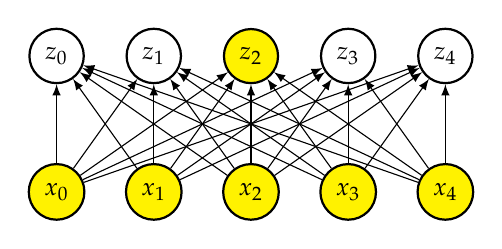
\begin{tikzpicture}[auto,node distance=8mm,>=latex,font=\small]
	
	\tikzstyle{round}=[thick,draw=black,circle]
	
	\node[round, fill=yellow] (x2) {$x_2$};
	\node[round,left=5mm of x2, fill=yellow] (x1) {$x_1$};
	\node[round,left=5mm of x1, fill=yellow] (x0) {$x_0$};
	\node[round,right=5mm of x2, fill=yellow] (x3) {$x_3$};
	\node[round,right=5mm of x3, fill=yellow] (x4) {$x_4$};
	\node[round,above=10mm of x0] (z0) {$z_0$};
	\node[round,above=10mm of x1] (z1) {$z_1$};
	\node[round,above=10mm of x2, fill=yellow] (z2) {$z_2$};
	\node[round,above=10mm of x3] (z3) {$z_3$};
	\node[round,above=10mm of x4] (z4) {$z_4$};
	
	\draw[->] (x0) -- (z0);
	\draw[->] (x0) -- (z1);
	\draw[->] (x0) -- (z2);
	\draw[->] (x0) -- (z3);
	\draw[->] (x0) -- (z4);
	\draw[->] (x1) -- (z0);
	\draw[->] (x1) -- (z1);
	\draw[->] (x1) -- (z2);
	\draw[->] (x1) -- (z3);
	\draw[->] (x1) -- (z4);
	\draw[->] (x2) -- (z0);
	\draw[->] (x2) -- (z1);
	\draw[->] (x2) -- (z2);
	\draw[->] (x2) -- (z3);
	\draw[->] (x2) -- (z4);
	\draw[->] (x3) -- (z0);
	\draw[->] (x3) -- (z1);
	\draw[->] (x3) -- (z2);
	\draw[->] (x3) -- (z3);
	\draw[->] (x3) -- (z4);
	\draw[->] (x4) -- (z0);
	\draw[->] (x4) -- (z1);
	\draw[->] (x4) -- (z2);
	\draw[->] (x4) -- (z3);
	\draw[->] (x4) -- (z4);
	\end{tikzpicture}
	\caption{A normal feedforward network}
	\label{connected}
\end{figure}

In a regular feedforward network, every output node, such as $z_2$, is affected by every input node, as seen by the shaded nodes in figure \ref{connected}.

\begin{figure}[h]
	\centering
	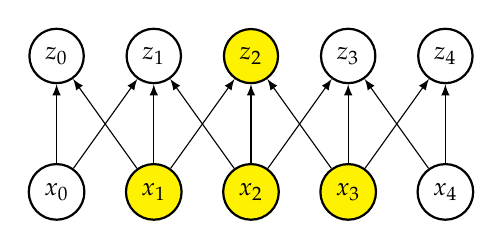
\begin{tikzpicture}[auto,node distance=8mm,>=latex,font=\small]
	
	\tikzstyle{round}=[thick,draw=black,circle]
	
	\node[round, fill=yellow] (x2) {$x_2$};
	\node[round,left=5mm of x2, fill=yellow] (x1) {$x_1$};
	\node[round,left=5mm of x1] (x0) {$x_0$};
	\node[round,right=5mm of x2, fill=yellow] (x3) {$x_3$};
	\node[round,right=5mm of x3] (x4) {$x_4$};
	\node[round,above=10mm of x0] (z0) {$z_0$};
	\node[round,above=10mm of x1] (z1) {$z_1$};
	\node[round,above=10mm of x2, fill=yellow] (z2) {$z_2$};
	\node[round,above=10mm of x3] (z3) {$z_3$};
	\node[round,above=10mm of x4] (z4) {$z_4$};
	
	\draw[->] (x0) -- (z0);
	\draw[->] (x0) -- (z1);
	\draw[->] (x1) -- (z0);
	\draw[->] (x1) -- (z1);
	\draw[->] (x1) -- (z2);
	\draw[->] (x2) -- (z1);
	\draw[->] (x2) -- (z2);
	\draw[->] (x2) -- (z3);
	\draw[->] (x3) -- (z2);
	\draw[->] (x3) -- (z3);
	\draw[->] (x3) -- (z4);
	\draw[->] (x4) -- (z3);
	\draw[->] (x4) -- (z4);
	\end{tikzpicture}
	\caption{Sparse connectivity in a CNN}
	\label{sparse}
\end{figure}

However, for a CNN layer (with a kernel width of 3 in this case), each output node is only affected by 3 input nodes, as seen in figure \ref{sparse}. This reduces memory requirements and increases computational efficiency, while allowing complex interactions between different pixels of an image to still be described. Furthermore, a CNN employs parameter sharing. While in regular feedforward networks every parameter is only used once, the smaller kernel means that its set of parameters only need to be learned once and is applied to all parts of the image. This makes the training phase require much less memory and is more efficient at describing transformations which apply across the entire image. 

The fact that convolution has equivariance, where changes in the input will affect the output in the same way, allows CNNs to efficiently map the region of features in the 2-D input to the 2-D output. This will be essential when computing attention over specific parts of the image in section \ref{extensions}. For these reasons, CNNs will be chosen as a means of understanding the image in this task.

\subsection*{The Recurrent Neural Network (RNN)}
RNNs are similar to feedforward networks, except that loops occur on some nodes, as shown in figure \ref{rnnNode}. They are specialized for taking in sequences of input values, as each increment on t can process a new chunk of input.

\begin{figure}[h]
	\centering
	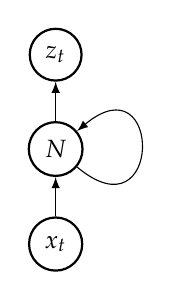
\begin{tikzpicture}[auto,node distance=8mm,>=latex,font=\small]
	
	\tikzstyle{round}=[thick,draw=black,circle]
	
	\node[round] (N) {$N$};
	\node[round,above=5mm of N] (z) {$z_t$};
	\node[round,below=5mm of N] (x) {$x_t$};
	
	\draw[->] (N) -- (z);
	\draw[->] (x) -- (N);
	\draw[->] (N) [out=-40,in=40,loop] to coordinate[pos=0.1](aa) (N);
	\end{tikzpicture}
	\caption{A node in a Recurrent Neural Network}
	\label{rnnNode}
\end{figure}
These loops allow information taken from one time step to persist to future states, which is important when dealing with a question with different parts relating to each other. However, regular RNNs face the problem of long term dependencies, and would not do well in learning questions where the context and subject may be far apart. For example, a question such as, “There is a sad person in the picture. Is this person male or female?” has the context of a “sad person” being a distance away from the subject of whether the person is male or female. In practice, an RNN has been shown as unable to handle such long-term dependencies well. As such, the project will instead use a different variation of the RNN, called the Long Short-Term Model (LSTM) for this task.


\subsection*{The Long Short-Term Memory Model (LSTM)}
The LSTM is similar in structure to the RNN above, except that each recurrent node has the structure shown in fig \ref{fig:lstm}.\footnotetext{Image from  http://colah.github.io/posts/2015-08-Understanding-LSTMs/}
\begin{figure}[h]
	\centering
	\includegraphics[width=0.5\linewidth]{lstm}
	\caption{An LSTM node\protect\footnotemark}
\label{fig:lstm}
\end{figure}
By default, they specialize in being able to learn long-term dependencies\cite{LSTM}. The rectangular nodes here represent neural network layers while the X represents the pointwise multiplication operation. The combination of the 2 is called a gate, which controls how much information to let through and what information to forget. This allows much longer term dependencies to be learned.

Since the questions in the VQA dataset are a sequence of text, often with multiple subjects in the question, they are best handled by an LSTM. These can be used to process the question by taking in a word at each time step.

\subsubsection{Visual QA Models}\label{models}
The models described below will be implemented and investigated as part of the core project and evaluated on the VQA dataset. Although a number of different models to be investigated are listed here, the project will also look at optimization and regularization techniques within each of these architectures. 

\paragraph{BOW+IMG Model}\label{bowimg}

This model takes the approach of embedding the question using a single Bag-Of-Words (BOWs) vector. For the image, GoogLeNet's pre-trained model will be used to extract its features and transform it into a feature vector. These 2 vectors will be concatenated and fed into a softmax layer to predict the answer class. This structure is shown in figure \ref{fig:bowimg3}. It is also used as a baseline model.

\begin{figure}[h]
\centering
\includegraphics[width=0.8\linewidth]{BOWIMG3}
\caption{Architecture of the BOW+IMG model}
\label{fig:bowimg3}
\end{figure}
Making use of BOWs to embed the question ignores the structure of the question, but it can still identify its main topics. GoogLeNet's model is trained on general images and not on the Visual QA task, hence it is not expected to provide an ideal performance. However, both of these provide a quick working model as a starting implementation which can be investigated and improved.

\subsubsection{LSTM+IMG Model}\label{LSTM+CNNModel}
This model will also use GoogLeNet for extracting the image features. However, instead of using the BOW model to input the question as a sequence, it will use an LSTM. The input at each time step of the LSTM will be one word of the question, concatenated with the encoded image vector, as shown in figure \ref{fig:ayn1}. 
\begin{figure}[h]
\centering
\includegraphics[width=0.7\linewidth]{AYN1}
\caption{Architecture of the LSTM+IMG model}
\label{fig:ayn1}
\end{figure}
The LSTM blocks in the figure show how the nodes look when they are rolled out, taking in one word each time together with the image vector. To produce an answer, the model is used to predict a sequence of output over a vocabulary, which is shown by the softmax layer after the full sequence is processed. This model will follow an architecture similar to \cite{CNNLSTM}. As a start, this vocabulary will consist of the 1000 most frequent answers in the VQA dataset. Further approaches for deciding this vocabulary will also be investigated in the extended models.

As described in section \ref{architect}, LSTMs are the state-of-the-art algorithms for processing natural language, and their strengths make them a reasonable choice for use in understanding the question text. This model aims to utilise the LSTM and image features, combined with a softmax layer, to understand the question, image and produce an answer from both.

This architecture can be further built upon by experimenting with the depth and width of the layers, as well as using regularization techniques to reduce overfitting.

\subsection{Extensions}\label{extensions}
The following extensions will be implemented if time permits, but are not crucial to the core of the project. 
\subsubsection{LSTM+CNN trained on VQA}\label{CNNonVQA}
All CNN models in the core project till this point have used a pre-trained model on ImageNet. While these are great at general classification, they have not been tuned towards the Visual QA task. This extension will implement its own CNN architecture and train it on the \href{http://www.image-net.org/}{ImageNet dataset}\footnote{http://www.image-net.org/}. Next, it will randomly initialize and train the last layer of the CNN model together with the LSTM on the VQA task. This will make use of the same model structure as \ref{LSTM+CNNModel}, but with its own CNN trained on the VQA task together with the LSTM, instead of training the LSTM separately.

\subsubsection{Attention over the image}
Standard neural network architectures often fail to produce precise answers if they require looking at a fine-grained region of an image. A higher level of reasoning is required for many of the VQA questions in order to pinpoint relevant parts of an image which are related to the question. Making use of Stacked Attention Networks (SAN) greatly improves this aspect\cite{SAN}.

SANs are generally made up of 3 components. The first is a method for image encoding. My implementation will make use of the CNN model trained in section \ref{CNNonVQA}, and the image features will be extracted from its last pooling layer so that the image spatial information is retained. The next component is the question model. My implementation will make use of the same LSTM architecture used in the previous section.

The output from these 2 components will be an image feature matrix, $V_i$ and a question feature vector, $V_q$. Both of these are fed into a single layer neural network and then through a softmax layer. Up to this point, the architecture can be described by figure \ref{fig:attentionimg}.
\begin{figure}[h]
\centering
\includegraphics[width=0.7\linewidth]{attentionImg}
\caption{Computing the first attention distribution}
\label{fig:attentionimg}
\end{figure}


The output of the softmax layer is an attention distribution, which is used to calculate the weighted sum of the initial image vectors, $V_i$. By combining this with $V_q$, we attain a new query vector U. This process of computing a new query vector can be iterated multiple times to enhance the attention over an image. My implementation will calculate the attention vectors twice before feeding it into a softmax layer to produce an answer to the question.

\subsubsection{Attention over the question}
Just as it is important to pinpoint parts of the image to give importance to, giving attention to parts of the question can be equally as important\cite{coAtt}. This architecture builds upon the previous section by making use of question attention on top of image attention. 
\begin{figure}[h]
\centering
\includegraphics[width=0.7\linewidth]{attentionQn1}
\caption{Question Encoding for the Question Attention Network}
\label{fig:attentionqn1}
\end{figure}
The main structure of the network is similar to the previous sections, except that the encoding of the question is done through the architecture shown in Figure \ref{fig:attentionqn1}, which begins by attaining word level features from the embedded vector space, before a 1-D convolution is applied to compute phrase level features, and subsequently question level features from the LSTM. 

At each step of this hierarchy, the attention weight, \textbf{H}, of a feature X,  is computed through equation \ref{hech} and \ref{ax}.

\begin{equation}\label{hech}
\textbf{H} = tanh(\textbf{WX} + (\textbf{Wg})1^\top)
\end{equation} 
\begin{equation}\label{ax}
\textbf{a}^x = softmax(\textbf{w}^\top H)
\end{equation}
W refers to the weights, while 1 refers to a vector with all elements as 1. g refers to an intermediate attention matrix, since this approach of computing attention over the question can be iterated together with computing attention over the image multiple times.

Once attention is computed, a feedforward network will be used to encode the attention features and the softmax output units will be used to produce an answer.

\subsubsection{Building a web interface.}
This will be done using the Flask framework which calls one of the implemented models. The model will be pre-trained offline before it is uploaded onto a server. A Graphical User Inferface (GUI) will allow anyone using the site to ask questions on displayed images, which will be sent as input to the model, and an answer will be returned.

\subsection{Evaluation}

The VQA datasets provide fully labelled training and validation sets, containing 248,349 and 121,512 questions respectively for the real images set. The testing procedures in this project will follow that in \cite{SAN} to allow a comparison with their result: the validation set will be equally split into Val1 and Val2. The training set and Val1 will be used for training and validating the models in this project. Val2 will be used for testing the models and for providing an in-depth analysis. Each answer from the dataset and the model will be normalised (e.g. all lowercase, no punctuation) and checked for equality to get a result on correct answers. 

The dataset includes two types of images, abstract and real-world, and two types of question formats, multiple-choice and open-ended. The evaluation will focus on using MSCOCO images, which are the real-world images. 

If time permits, the Abstract image set will also be used for an additional level of evaluation. Abstract images reduce the need to handle noise, so the models will focus more heavily on higher level reasoning. A varied performance between models on abstract and real-world datasets can help to distinguish between result improvements due to noise handling or improved reasoning. Multiple choice and open-ended questions can also help to evaluate the generative parts of the model. Furthermore, the questions can be clustered into types such as "What" or "Why" questions, and differences in the performance on different question types will aid in directing further improvements, such as whether the question type might require prior knowledge.

For the multiple-choice questions, the models will be evaluated on the percentage of answers which they are able to get correct. For the open-ended answers, they will also be evaluated on percentage of answers which are equal to the ground truth answer, but on top of this, the similarity of the answer produced to the ground truth answer will also be taken into account using the word2vec similarity score.

\subsection{Dissertation Writeup}
In order to ensure the results and challenges faced in the project are adequately remembered and documented, the writing of the dissertation and implementation of the project will happen concurrently. Early drafts of the dissertation will be written in point form for the purpose of quick recording. As the project nears completion, this will be expanded upon and formalised.

\section{Success Criteria}
\subsection{Main Project}
The project will be evaluated upon the following success criteria:
\setlength{\parskip}{0em}
\begin{enumerate}
	\item Implement a Visual QA Model which embeds its question input using BOW and a pre-trained model to extract image features, and is able to produce a text answer to each question in the test set.
	\item Implement a Visual QA Model which uses an LSTM for embedding the question, and a pre-trained CNN to extract image features, and is able to produce a text answer to each question in the test set.
	\item An evaluation done between 1) and 2) which produces comparative statistics on their accuracy and percentage of correct answers on the test set.
\end{enumerate}
\setlength{\parskip}{1em}
\subsection{Extensions}
For the extensions, the following success criteria apply:
\setlength{\parskip}{0em}
\begin{enumerate}
	\item Train a CNN and implement a model using it which can produce a text answer to each question in the test set.
	\item Implement a model which uses attention over an image to produce a text answer for each question in the test set.
	\item Implement a model which uses attention over an image and question to produce a text answer for each question in the test set.
	\item Create a web interface which can take an image and question query, call one of these models and return its answer.
\end{enumerate}
\setlength{\parskip}{1em}

\section{Resource Required}
\subsection{Machines}
I will use my personal laptop, a Dell XPS 13 (9343) with 2.4GHz Intel Core i7 CPU and 8GB RAM, dual booted with Ubuntu and Windows 8.1, for the development of this project. I accept full responsibility for this machine and I have made contingency plans to protect myself against hardware and/or software failure.

In order to protect against hardware and/or software failures, the following measures will be taken:
\setlength{\parskip}{0em}
\begin{itemize}
	\renewcommand{\labelitemi}{\textbullet}
	\item All code will be regularly pushed into my project repository on Github for revision control.
	\item All relevant documents and code will be regularly synchronised, as well as manually uploaded, to my Google Drive and Dropbox.
	\item An external hard disk will also be used to regularly back up all project files.
\end{itemize}

For training of the models, the University's High Performance Computing Service will be used. I have contacted my supervisor, Dr Marek Rei, for this and the relevant permission for using this has been granted.

\setlength{\parskip}{1em}

\subsection{Tools}\label{Tools}

\textbf{Tensorflow:} an open source software library for machine intelligence, to implement the neural network architectures. While building neural network architectures from scratch is possible, the aim of the project is to investigate architectures for building a Visual QA system, rather than on constructing neural networks. Thus, Tensorflow will be used for this. It is also commonly used in industry and distributes computations well to Graphics Processing Units(GPUs), and hence I would like to learn more about it. 

\href{http://www.nltk.org/}{\textbf{NLTK}}\footnote{http://www.nltk.org/}\textbf{:} A Natural Language Toolkit. It will be used for tasks such as tokenization in preparing the question datasets for Tensorflow.

\href{https://www.tensorflow.org/tutorials/word2vec}{\textbf{word2vec}}\footnote{https://www.tensorflow.org/tutorials/word2vec}\textbf{:} A model used to produce word embeddings. It will be used for calculating the similarity between words for evaluating open-ended answers.

\textbf{GoogLeNet or VGGNet model:} Both of these are Deep CNNs pre-trained on ImageNet\cite{CNN}. Depending on their performance and whether it is possible to access intermediate layer values, one of these will be used to extract image features for the 2 models in the core project. \href{http://caffe.berkeleyvision.org/}{Caffe}\footnote{http://caffe.berkeleyvision.org/} may also be used for running these models.

\href{http://flask.pocoo.org/}{\textbf{Flask}}\footnote{http://flask.pocoo.org/}\textbf{:} A micro web framework for Python. It will be used for building the web interface for the model.


\subsection{Datasets}

The \href{http://visualqa.org/vqa_v1_download.html}{VQA dataset}\footnote{http://visualqa.org/vqa\_v1\_download.html} provides a large and labeled corpus of images, questions and the answers to those questions in JSON format.
It is publicly available and is free to adapt and share under the Commons Attribution 4.0 International License.

Each dataset is downloaded in 3 separate parts:
\setlength{\parskip}{0em}
\begin{enumerate}
	\item  Question set in JSON, contains the question, question ID and image ID
	\item Image set containing the image in png format, named with the image ID
	\item Annotations set in JSON, containing the question type, answer type, question ID, image ID and 10 ground truth answers.
\end{enumerate}
Image and Question IDs allow questions, images and answers to be mapped to each other.
The dataset does not provide any extracted features, just questions in JSON string and images in png.
\setlength{\parskip}{1em}

For real world images, there are 248,349 training questions and 121,512 validation questions. With these, there are 82,783 training images and 40,504 validation images. For abstract scenes, there are 60,000 training questions and 30,000 validation questions. These are accompanied by 20,000 training images and 10,000 validation images. All of these are fully labelled.

Each image has an average of 3 questions about it, and each question has 10 ground truth answers. Since the 10 answers were annotated by Amazon Mechanical Turk (AMT), not all of them may be accurate. For evaluating this project, a majority vote (with tie breaker measures) will be performed on the 10 ground truth answers to attain the most certain answer for checking. 

\section{Timetable and Milestones}

The project will be split into two-week sprints. While it is difficult to get an accurate measure of my sprint rate, the milestones and deliverables for each two-week block will be stated as tangibly as possible, so they can be evaluated and adjusted accordingly for the following sprint. Below is my initial estimation of the timetable for this project.

\setlength{\parskip}{1em}
\renewcommand\labelitemi{\textasteriskcentered}

\noindent\textbf{Sprint 1: Michaelmas week 3-4 (19 October - 1 November)}
\begin{addmargin}[3em]{0em}
		\noindent\textbf{Project Proposal Deadline: 20 October}
		\setlength{\parskip}{0em}
	\begin{itemize}
		\setlength\itemsep{0em}
		\item Set up and get familiar with Python and Tensorflow 
		\item Do the online Udacity Deep Learning Course 
		\item Read papers on the visual question answering task and on each of the architectures that I plan on implementing, and refer to the deep learning textbook for how these can be implemented
		\item Download all datasets to be used and split them into training, validation and test sets
	\end{itemize}
	\setlength{\parskip}{0em}
	\noindent\textbf{Milestone:} Python and Tensorflow set up; simple programs written to test it is working; Notes made on the overall structure of the models to implement.
	\vspace{1em}
\end{addmargin}
\newpage
\noindent\textbf{Sprint 2: Michaelmas week 5-6 (2 November - 15 November)}
\begin{addmargin}[3em]{0em}
	\begin{itemize}
		\setlength\itemsep{0em}
		\item Implement a skeleton structure of the program which can read VQA input
		\item Implement a component which can convert VQA question input into BoWs
		\item Implement a component which can extract image features from the VQA image input
		\item Continue reading up on LSTMs and CNNs for the next architecture
	\end{itemize}
		\noindent\textbf{Milestone:} Skeleton structure of the program written; Working components for BOW and image extraction.
		\setlength{\parskip}{1em}
\end{addmargin}	

\noindent\textbf{Sprint 3: Michaelmas week 7-8 (16 November - 29 November)}
\setlength{\parskip}{1em}
\begin{addmargin}[3em]{0em}
	\begin{itemize}
		\setlength\itemsep{0em}
		\item Complete the BOW+IMG model which integrates the previous 3 components and begin training it
		\item Build a test harness around the starting model and attain first set of results for the baseline
		\item Begin reading up and experimenting with LSTMs and CNNs
	\end{itemize}
	\noindent\textbf{Milestone:} Training for BOW+IMG model has started.
	\setlength{\parskip}{1em}
\end{addmargin}

\noindent\textbf{Sprint 4: Michaelmas Vacation week 1-2 (30 November - 13 December)}
\begin{addmargin}[3em]{0em}
	\begin{itemize}
		\setlength\itemsep{0em}
		\item Build the LSTM component for the LSTM+CNN model
		\item Test the BOW+IMG model on the VQA dataset
		\item Complete the implementation for the LSTM+CNN model and begin training
	\end{itemize}
	\noindent\textbf{Milestone:} Attain a set of results from the BOW+IMG model
	\setlength{\parskip}{1em}
\end{addmargin}

\noindent\textbf{Sprint 5: Michaelmas Vacation week 3-4 (14 December - 27 December)}
\begin{addmargin}[3em]{0em}
	\begin{itemize}
		\setlength\itemsep{0em}
		\item Buffer for any remaining implementation
		\item Start writing Introduction, Preparation and Conclusion chapters of dissertation
	\end{itemize}
	\noindent\textbf{Milestone:} Draft of 3 chapters prepared; LSTM+IMG model began training
	\setlength{\parskip}{1em}
\end{addmargin}

\noindent\textbf{Sprint 6: Michaelmas Vacation week 5-6 (28 December  - 10 January)}
\begin{addmargin}[3em]{0em}
	\begin{itemize}
		\setlength\itemsep{0em}
		\item Test the LSTM+IMG model
		\item Evaluate the 2 models to get a set of comparative results
		\item Read and begin experimenting on training CNN models
		\item Tweak the architecture of the models and conduct tests to investigate ways of improving results
	\end{itemize}
	\noindent\textbf{Milestone:} Attain a set of results from the LSTM+IMG model
	\setlength{\parskip}{1em}
\end{addmargin}
\newpage
\noindent\textbf{Sprint 7: Michaelmas Vacation / Lent week 1 (11 January - 24 January)}
\begin{addmargin}[3em]{0em}
	\begin{itemize}
		\setlength\itemsep{0em}
		\item Implement and begin training the CNN extension model
		\item Write a draft of the progress report
	\end{itemize}
	\noindent\textbf{Milestone:} Draft of progress report submitted for feedback; CNN extension model started training 
	\setlength{\parskip}{1em}
\end{addmargin}

\noindent\textbf{Sprint 8: Lent week 2-3 (25 January - 7 February)}
\begin{addmargin}[3em]{0em}
	\noindent\textbf{Progress Report Deadline: 2 February}
	\setlength{\parskip}{0em}
	\begin{itemize}
		\setlength\itemsep{0em}
		\item Test the CNN extension model and evaluate with the other models
		\item Read up on attention-models and begin building the attention over images model
		\item Complete and submit the progress report
	\end{itemize}
	\noindent\textbf{Milestone:} Progress report submitted; Attain set of results from CNN extension model
	\setlength{\parskip}{1em}
\end{addmargin}

\noindent\textbf{Sprint 9: Lent week 4-5 (8 February - 21 February)}
\begin{addmargin}[3em]{0em}
	\begin{itemize}
		\setlength\itemsep{0em}
		\item Complete and begin training for the attention over images model
		\item Research on attention over text
		\item Write a draft of implementation and evaluation chapters of dissertation
	\end{itemize}
	\noindent\textbf{Milestone:} Implementation and evaluation chapters draft ready
	\setlength{\parskip}{1em}
\end{addmargin}

\noindent\textbf{Sprint 10: Lent week 6-7 (22 February - 7 March)}
\begin{addmargin}[3em]{0em}
	\begin{itemize}
		\setlength\itemsep{0em}
		\item Begin implementing the attention over question model
		\item Test the attention over images model
		
	\end{itemize}
	\noindent\textbf{Milestone:} Attain a set of results for the attention over images model
	\setlength{\parskip}{1em}
\end{addmargin}

\noindent\textbf{Sprint 11: Lent week 8 / Easter Vacation (8 March - 21 March)}
\begin{addmargin}[3em]{0em}
	\begin{itemize}
		\setlength\itemsep{0em}
		\item Complete and begin training the attention over question model
		\item Begin writing a full draft of dissertation
	\end{itemize}
	\noindent\textbf{Milestone:} Submit introduction and preparation chapters to DOS
	\setlength{\parskip}{1em}
\end{addmargin}

\noindent\textbf{Sprint 12: Easter Vacation week 2-3 (22 March - 4 April)}
\begin{addmargin}[3em]{0em}
	\begin{itemize}
		\setlength\itemsep{0em}
		\item Buffer block for any remaining implementation
		\item Do a final test and evaluation over all models
		\item Complete draft of dissertation, submit to DOS and amend accordingly
		\item Begin on second draft
	\end{itemize}
	\noindent\textbf{Milestone:} Draft submitted to DOS; All code for implementations completed
	\setlength{\parskip}{1em}
\end{addmargin}

\noindent\textbf{Sprint 13: Easter Vacation week 4-5 (5 April - 18 April)}
\begin{addmargin}[3em]{0em}
	\begin{itemize}
		\setlength\itemsep{0em}
		\item Complete second draft, get feedback and amend accordingly
		\item Revision for written papers
	\end{itemize}
	\noindent\textbf{Milestone:} Second draft completed
	\setlength{\parskip}{1em}
\end{addmargin}

\noindent\textbf{Sprint 14: Easter Vacation / Easter week 1 (19 April - 2 May)}
\begin{addmargin}[3em]{0em}
	\begin{itemize}
		\setlength\itemsep{0em}
		\item Prepare final dissertation draft - get feedback, proofread, amend and iterate
		\item Submit final draft for feedback
		\item Revision for written papers
	\end{itemize}
	\noindent\textbf{Milestone:} Final draft completed
	\setlength{\parskip}{1em}
\end{addmargin}

\noindent\textbf{Sprint 15: Easter week 2-3 (3 May - 16 May)}
\begin{addmargin}[3em]{0em}
	\begin{itemize}
		\setlength\itemsep{0em}
		\item Final touching up on any further dissertation comments 
		\item Revision for written papers
	\end{itemize}
	\noindent\textbf{Milestone:} Submit Dissertation
	\setlength{\parskip}{1em}
\end{addmargin}

\setlength{\parskip}{1em}
\noindent\textbf{Deadline: 18 May}
\vspace{1em}

\newpage
\bibliographystyle{abbrv}
\bibliography{biblio}


 
 

%----------------------------------------------------------------------------------------

\end{document}
